\documentclass[10pt, a4paper]{article}
\usepackage{lrec}
\usepackage{multibib}
\newcites{languageresource}{Language Resources}
\usepackage{graphicx}
\usepackage{tabularx}
\usepackage{soul}
% for eps graphics

\usepackage{epstopdf}
\usepackage[utf8]{inputenc}

\usepackage[hidelinks]{hyperref}
\usepackage{xstring}

\usepackage{color}
\setlength{\parskip}{4pt}

\newcommand{\secref}[1]{\StrSubstitute{\getrefnumber{#1}}{.}{ }}


\usepackage{float}
\usepackage{listings}

\newfloat{lstfloat}{htbp}{lop}
\floatname{lstfloat}{Schema}
\def\lstfloatautorefname{Schema} % needed for hyperref/auroref

\lstset{
  basicstyle=\footnotesize\ttfamily
}

\title{\textbf{Enriching Historic Photography with Structured Data
using Image Region Segmentation}}

\name{Taylor Arnold\textsuperscript{$\dagger$}, Lauren Tilton\textsuperscript{*}}

\address{\textsuperscript{$\dagger$}Department of Mathematics and Computer Science, University of Richmond \\
  \textsuperscript{*}Department of Rhetoric and Communication Studies, University of Richmond \\
     410 Westhampton Way, Richmond, VA, USA 23173 \\
     \{tarnold2, ltilton\}@richmond.edu\\}

\abstract{
Cultural institutions such as galleries, libraries, archives and museums
continue to make  commitments to large scale digitization of collections.
An ongoing challenge is how to increase discovery and access through structured
data and the semantic web. In this paper we describe a method for using computer vision
algorithms that automatically detect regions of
``stuff''---such as the sky, water, and roads---to produce rich and accurate
structured
data triples for describing the content of historic photography.
We apply our method to a collection of 1610 documentary photographs
produced in the 1930s
and 1940 by the FSA-OWI division of the U.S. federal government. Manual
verification of the extracted annotations yields an accuracy rate
of 97.5\%, compared to 70.7\% for relations extracted from object detection
and 31.5\% for automatically generated captions. Our method also produces a rich
set of features, providing more unique labels (1170) than either the captions
(1040) or object detection (178) methods. We conclude by describing directions
for a linguistically-focused ontology of region categories that can better
enrich historical image data. Open source code and the extracted metadata from
our corpus are made available as external resources. \\
\newline \Keywords{computer vision, image segmentation, cultural heritage,
photography, Linked Data, ontology, digital humanities}
}

\begin{document}

\maketitleabstract

\section{Introduction}

Galleries, libraries, archives, and museums (known as GLAM institutions) and
other cultural heritage organizations have
increasingly sought to provide structured metadata about historic collections
in an effort to increase access and discovery. Where records have been
digitized and rights restrictions allow for it, many of these organizations
have also been able to make the digital records directly accessible through
openly available APIs and URIs. Prominent examples of these efforts include the
Rijksmuseum's \textit{RijksData} \cite{dijkshoorn2018rijksmuseum}, Europeana's
Search API, Record API, and SPARQL endpoint \cite{concordia2009not}, and the
\textit{Linked Data Service} provided by the United States Library of Congress
\cite{zimmer2015twitter}. The effort to make resources available
within a cohesive semantic web offers exciting possibilities for research and
public access to cultural collections. Yet, challenges remain for producing
structured data that facilitates access and exploration of digital archives.

Many digital collections held by cultural heritage organizations consist of
still and moving image data. These include scans of textual documents,
photographs of material culture, and digital scans of artwork,
photographs and other visual objects. Unlike machine-readable textual archives,
visual collections do not immediately offer a simple method for automated
search or data extraction. While records may include extensive metadata
about the provenance of a digital image, there is often little to no structured data
pertaining to the content of the image itself. Even when descriptive captions
exist, these are typically short and intended to be read alongside the object itself.
In other words, captions are written assuming that the reader will be able to look
at the object. The lack of
structured linguistic descriptions serves as a roadblock to providing rich links
between and across collections, as well as limiting the possibilities for
large-scale analysis. While expert and crowd-sourced annotations
can fill in some gaps, manual data construction requires extensive resources
and becomes more difficult as digitized datasets increase in size
\cite{seitsonen2017crowdsourcing}.

\begin{figure*}[!ht]
\begin{center}
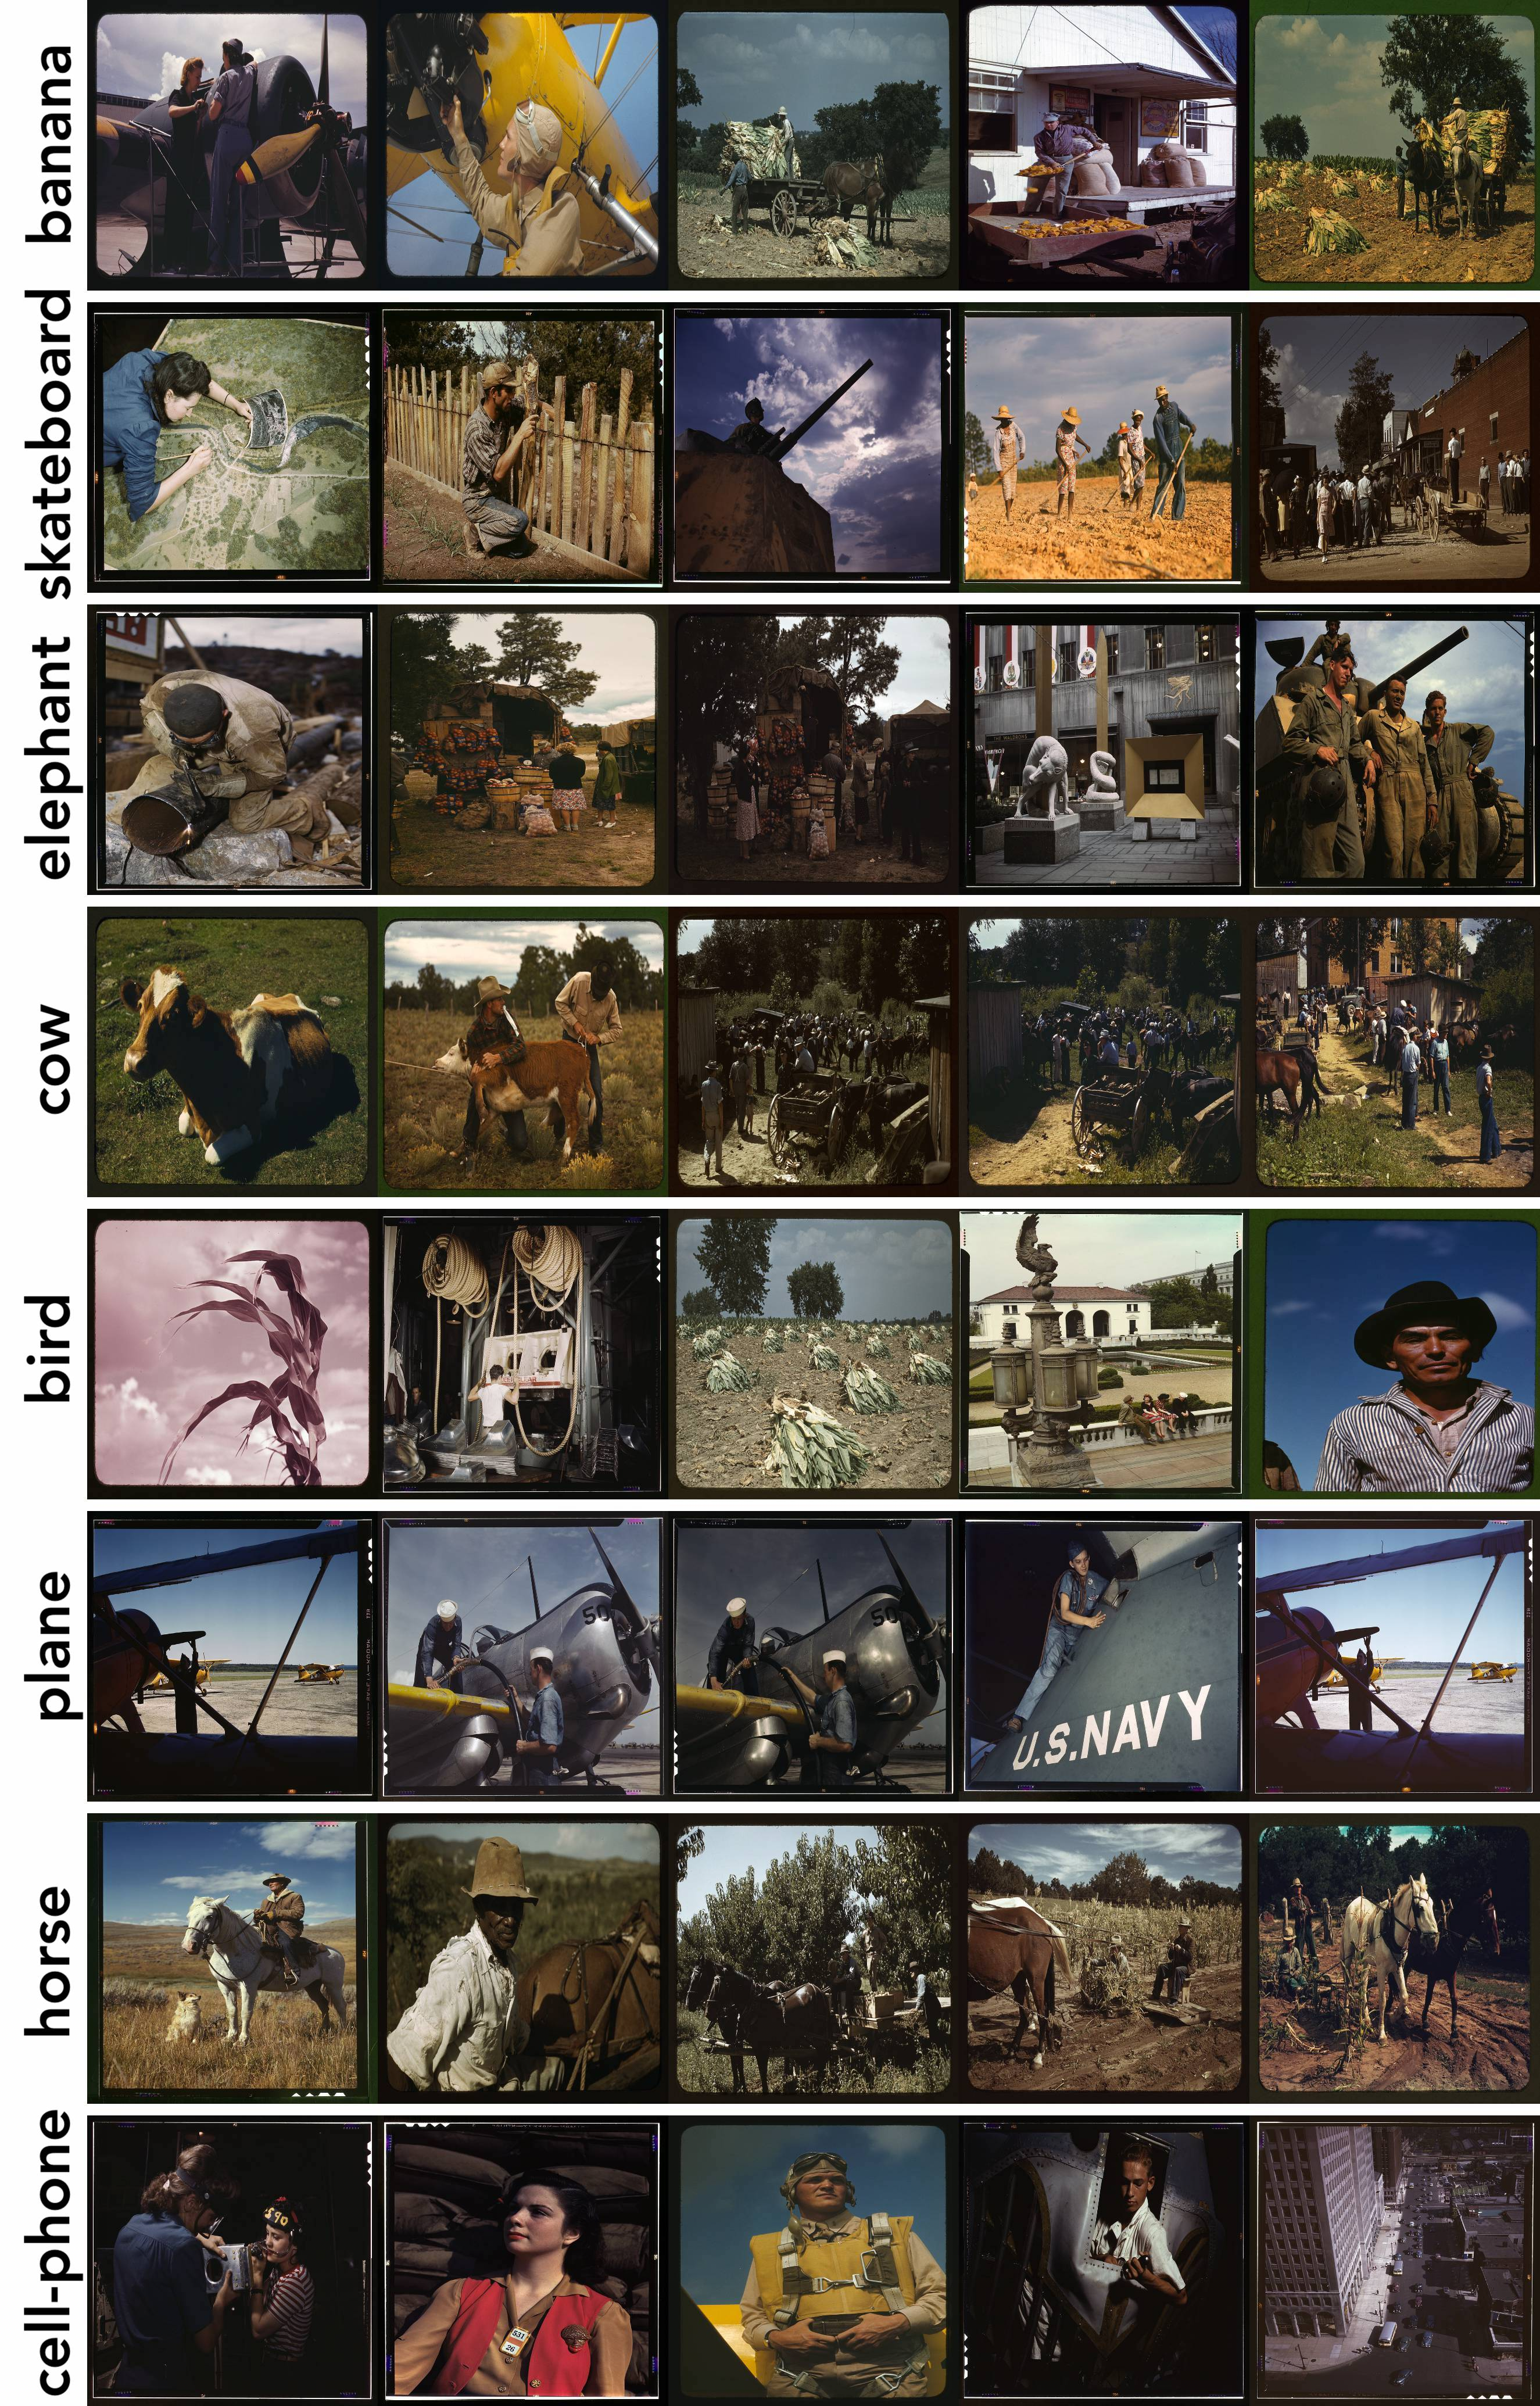
\includegraphics[width=0.82\textwidth]{../figures/max_things_grid_labels.jpg}
\caption{Automatically generated labels assigned to FSA-OWI color photographs
by the Mask R-CNN instance object classification algorithm (X101-FPN)
\protect\cite{wu2019detectron2}. For each of the eight selected object types,
the five images from the FSA-OWI color
photographs that are most predicted to contain the given category are shown.
All categories were estimated to exist with probability greater than 80\%. The
plane and horse categories seem to have correctly identified the objects in
their five respective images, and two of the cow images are in fact cows
(the others are horses). The remaining categories seem to be all false
detections. Many mistakes are hard to explain, such as the row of skateboard
objects.
}
\label{fig:things}
\end{center}
\end{figure*}

\begin{figure*}[!ht]
\begin{center}
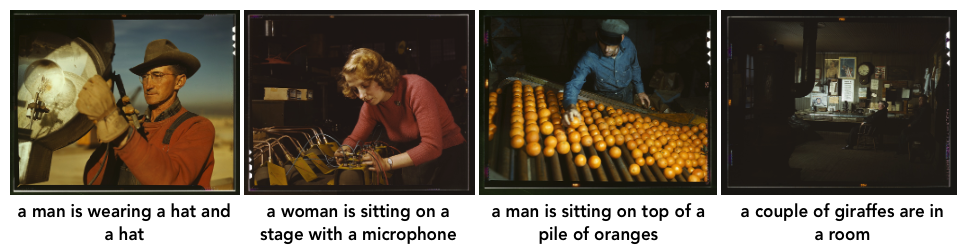
\includegraphics[width=0.95\textwidth]{../figures/captions.png}
\caption{Three detected captions for three FSA-OWI photographs using the
`Show, attend and tell' model \protect\cite{xu2015show}. The first provides a
caption that matches the image and the third produces a caption that is very
similar to the image. The second correctly identifies the subject of a woman
in the frame but mistakenly believes she is holding a microphone. The final
image produces an annotation that incorrectly labels the people as giraffes.}
\label{fig:captions}
\end{center}
\end{figure*}

Computer vision techniques provide a direction for the automated creation of
structured data to enrich collections of historic digital images. Machine
learning techniques can detect features present in images and store these
alongside human-generated metadata pertaining to the digital records. However,
the use of automated techniques have their own unique set of challenges. Most
computer vision algorithms are built using modern datasets, and may produce
annotations that are inaccurate or inappropriate for historic data. Incorrectly
extracted data records are particularly concerning when making data available
to the public. Even when including confidence scores for extracted features,
studies have shown that people have trouble accurately interpreting probabilistic
data and are overly confident in predictions \cite{khaw2019individual}.
The challenges of mis-classified data are particularly acute when they risk
reinforcing racial, gender, and socioeconomic biases inherent in the training
data behind machine learning techniques. For example, a recent study showed
that face
detection algorithms have difficulty identifying darker skinned individuals
\cite{buolamwini2018gender}. Applying state-of-the-art face detection
algorithms to a collection of photographs, therefore, risks further hiding
marginalized communities.

In this article we present a method for the automated extraction of
highly-accurate structured data describing the content of historic photography
using computer vision algorithms. Specifically, our approach is based on the
detection of regions of the image containing elements described as ``stuff'',
which includes elements such as sky, water, trees, grass, and roads
\cite{caesar2018coco}. While temporal, cultural,
and regional differences  exist in some of these categories, the
stuff-based regions of images are significantly more robust than many other
features that can currently be extracted from image data.

We focus  on the application of our method to the 1610 color
photographs from the Farm Security Administration-Office of War Information
Collection (FSA-OWI) at the United States Library of Congress. We selected the
collection for three reasons. First, it is a part of one of the most famous and
researched photography archives from the United States \cite{tagg2009disciplinary}.
Second, the collection is held by a library that is invested in open access and
encourages experimentation with their digital collections. Third, the collection
is indicative of many documentary photography collections held in GLAM
institutions. It is a large enough collection that manual annotation of new
features would be overly time consuming and expensive. It has has some
descriptive metadata consisting of minimal captions, but these are too short and
vauge to easily facilitate semantic connections within and across
collections.

The remainder of this article is structured as follows.
Section~\secref{sec:background} gives a brief survey of several projects currently
using computer vision and structured data to augment historic image collections.
Section~\secref{sec:imageseg}  provides an overview of image segmentation and
the current approaches for the classification of stuff categories.
Section~\secref{sec:method} presents our specific approach and schema for
producing structured data from images. In Section~\secref{sec:eval} we give
an evaluation of our approach applied to a collection of 1610 photographs from the
1930s and 1940s. We conclude in Section~\secref{sec:conclude} with a discussion of
future possibilities and challenges of applying image segmentation to historic
datasets.


\section{Background} \label{sec:background}

The task of enriching image datasets with automated descriptions
has been approached from several angles. Methods include object detection (2.1),
automated captions (2.2) and image embeddings (2.3).
The objects of study in historic datasets often do not align with the
contemporary categories used to describe object detection algorithms,
automated captions, and the types of relationships produced by image
embeddings. Working with historic data to produce the kinds of automated
extraction of structured data necessary requires a different approach, which
we outline in the sections that follow.

\begin{figure*}[!ht]
\begin{center}
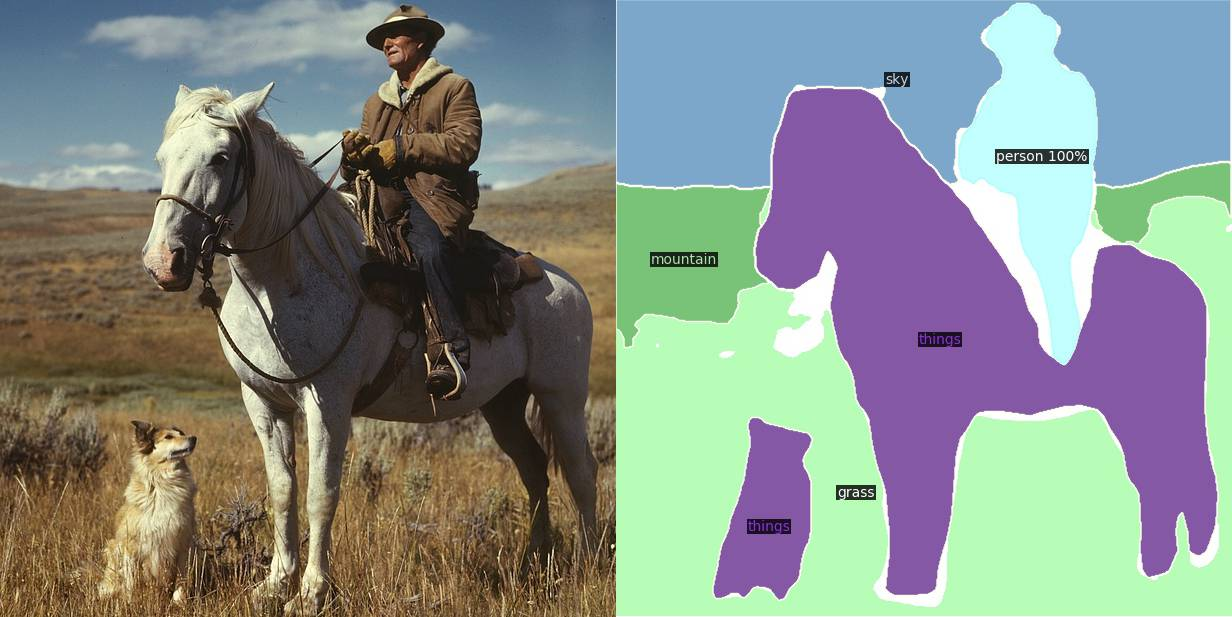
\includegraphics[width=0.95\textwidth]{../figures/segmentation_examples_small.jpg}
\caption{Example of a trained stuff-segementation algorithm applied to
one FSA-OWI photograph \protect\cite{wu2019detectron2}. The algorithm
detected five types of regions: sky, mountain, grass, things, and person.}
\label{tab:segmentation}
\end{center}
\end{figure*}

\subsection{Object Detection}

The algorithmic identification of objects within an image is one of the most
prominent tasks in computer vision. Early tasks focused on
relatively simple objectives, such as the classification of hand-written
digits in the MNIST dataset, which used small 28-by-28 grids of
black and white pixels
\cite{platt1999using}. Modern training datasets feature thousands of categories,
ranging for very specific categories, such as a specific species of dogs, to
relatively abstract concepts such as `grocery stores' and `parties'. Using
transfer learning, in which a model trained on one dataset is modified to
function on a new task, it is possible to produce algorithms trained to detect
virtually any object category by manually tagging only a small set of training
examples. The training of models for specific features has been employed in
the annotation of several historical image datasets, such as the location of
Dadaism art work \cite{thompson2017computational} and detecting figures in
digitized newspapers \cite{wevers2019visual}.

Current state-of-the-art models for detecting objects within images are difficult
to use as a general-purpose code system for the analysis of visual culture.
Available models feature categories that are too specific and only cover
a very small number of the object types that could be seen within the frame
of modern, western-centric film and photography. When considering historical
or more diverse datasets, the coverage is even worse. For example, the popular
ILSVRC dataset contains 1000 categories, but only seven types of fruits
(fig, pineapple, banana, pomegranate, apple, strawberry, orange, and lemon),
four vegetables (cucumber, artichoke, bell pepper, head cabbage), and eight
other food items (pretzel, bagel, pizza, hotdog, hamburger, guacamole, burrito,
and popsicle) \cite{russakovsky2015imagenet}. There are no generic catch-all
food categories for other items falling outside of these lists. While there are
120 subcategories for dog breeds, there is no category pertaining to horses or
cows. Applying these object detection models indiscriminately to a large corpus
without understanding its limitations will result in biased results. They will
find certain kinds of food items, animals, and clothing, but will completely
ignore examples outside of a narrowly curated  list of categories.

Object detection is a useful tool for annotating specific features of interest
within a collection. However, each feature requires a manually trained model
and may not generalize well to a new collection. Using existing models with
preselected categories on historic images typically produces a mix of
correct and false annotations. Figure~\ref{fig:things} shows the results
of a popular object detection algorithm to the FSA-OWI collection
\cite{wu2019detectron2}. While some categories produced reasonably accurate
annotations, such as the detection of horses and people, most categories detected
more false positives than successfully generated tags. Without a good general-purpose
collection of object detectors, a challenge discussed further in
Section~\secref{sec:conclude}, object detection remains difficult to use as a means
for producing structured data for linking historic image collections.

\subsection{Automated Captions}

Because object detection on its own has major challenges, particularly when
working with historic data, another method has been to use automated captions.
The automated generation of descriptive image captions is a more ambitious task
that has been a popular line of research at the intersection of computational
linguistics and computer vision. Captions generated through neural networks
with the help of linked
textual data have shown to be fairly accurate, offering a useful tool for
automated description of images in news articles and other media  powerful
\cite{hessel-etal-2019-unsupervised} \cite{BATRA18.725} \cite{HOLLINK16.19}.
As with object detection, automatically generated
captions within well-defined domains, such as profile photos, has also been
fairly successful at generating accurate descriptions \cite{GATT18.226}.
On the more general task of generating free-form image captions, current
state-of-the-art methods also produce impressive results when applied to
modern datasets \cite{nikolaus-etal-2019-compositional} \cite{jiang-etal-2019-reo}
\cite{wang-etal-2018-object}. On datasets that differ from the specific training data,
however, modern methods too-often produce nonsensical results that make them
difficult to deploy directly in an archive. Figure~\ref{fig:captions}
show the results of one popular caption algorithm applied to photographs from
the 1940s \cite{xu2015show}. While two captions produce reasonable results, a
third incorrectly identifies the object held by the main subject and the fourth
mistakenly believes the two men in the frame are giraffes.



\begin{table*}[ht!]
\centering
\begin{tabular}{lll}
 \hline
\textbf{Group} & \textbf{Meta Categories} & \textbf{Categories} \\
 \hline
 indoor & ceiling & ceiling-tile \\
 indoor & floor & floor-wood; floor-stone; floor-tile; floor-marble; carpet \\
 indoor & food & fruit; vegetable; salad \\
 indoor & furniture & cabinet; cupboard; counter; desk; door; light; mirror; shelf; stairs; table \\
 indoor & rawmaterial & cardboard; metal; paper; plastic \\
 indoor & textile & banner; blanket; curtain; cloth; clothes; napkin; mat; pillow; rug; towel \\
 indoor & wall & wall-brick; wall-stone; wall-tile; wall-wood; wall-panel; wall-concrete \\
 indoor & window & window-blind \\ \hline
 outdoor & building & bridge; house; roof; skyscraper; tent \\
 outdoor & ground & dirt; gravel; pavement; platform; playingfield; railroad; road; sand; snow; mud \\
 outdoor & plant & flower; grass; tree; bush; leaves; branch; moss; straw \\
 outdoor & sky & clouds \\
 outdoor & solid & mountain; rock; hill; stone; wood \\
 outdoor & structural & fence; net; railing; cage \\
 outdoor & water & river; sea; waterdrops; fog \\
  \hline
\end{tabular}
\caption{Hierarchical description of 91 stuff categories \protect\cite{caesar2018coco}.
Additionally, each metacategory other than ``rawmaterial'' also contains an
``other'' label (not shown) for regions that do not fit into any specific
category.}
\label{tab:categories}
\end{table*}

\subsection{Image Embedding}

Given the difficulty of automatically producing accurate structure data from
image collections, the use of image embedding has become a popular approach
for finding links between and across collections of visual data. Similar to
the process of using word embeddings, image embeddings most frequently project
a collection of images into the penultimate layer of a neural
network. Once represented as a sequence of numbers in a high-dimensional space,
images within an across collections can be associated with their closest
neighbors \cite{mcauley2015image}. Flattening image embeddings into two or three dimensions
produces useful visualizations of large image collections. Tools in the digital
humanities, such as Yale DH Lab's \textit{PixPlot}, make this approach
accessible to a large community of users and illustrates the appeal of its
method \cite{pixplot}.

For finding similar images or detecting patterns and trends within a collection,
image embeddings are a useful tool and generalize well to new and historic datasets.
By forgoing the explicit creation of structured data, they avoid many of the
pitfalls of the automated information extraction. However, the constructed data
does not produce meaningful relationships that can be easily distributed as
structured data. This makes it difficult to extend the recommendation system
to new collections and to find links across a web of archives.


\section{Image Segementation of Stuff} \label{sec:imageseg}

A recent development in computer vision has opened an exciting new path for the
automated description of images. In 2018, a research team from
University of Edinburgh and Google AI released a new corpus of image training
data that contained 91 new categories \cite{caesar2018coco}. However, unlike
previous image datasets, their categories did not focus on the detection of
specific objects. Rather, the team built an ontology and large collection of
training data to detect the ``amorphous background regions" within an image.
These regions do not correspond to objects, but instead to un-enumerable
collections such as the sky, water, and ceilings. The team described these
regions as ``stuff" categories and proposed a comprehensive ontology of them.
Their approach split all regions under two groups: ``indoor stuff" and
``outdoor stuff". These groups are further divided into meta categories,
which include ``water", ``ground", ``sky", ``furniture", and ``floor". Finally,
these are split into 91 fine-grained
categories such as ``sea", ``mud", ``clouds", and ``carpet". A full description
of the available categories is given in Table~\ref{tab:categories}.
The joint task of identifying these labels alongside object labels
has been one of shared tasks sponsored by the Common Objects in Context
challenge from 2017 to 2019 \cite{kirillov2019panoptic}.
As a result, there are now many accurate models for automatically labelling
these regions. Figure~\ref{tab:segmentation} shows the detected regions found
within an image from the FSA-OWI archive.

While no classification scheme
can be free of cultural assumptions nor account for all possible scenarios,
the stuff categories are significantly more generic than the object categories.
This is particularly true of the high- and mid-level categories. The
higher-level categories avoid some of the material-specific designations from
the lowest-level categories, such as wood flooring, that may not be applicable
with images that significantly depart from the available training data. By
aggregating information about detected stuff categories, we can make intelligent
guesses about whether an image was taken inside or outside, how the people in
the image are placed relative to the background, and the location and role of
the horizon in framing the image.

As always when working with automatically generated annotations, care should be
taken to avoid misinterpreting the results of stuff-segmentation algorithms.
There are categories that have a degree pf ambiguity between them, such as ``dirt"
and ``sand" or ``mat" and ``rug". Also, the stuff categories were designed
pragmatically for the task of assigning all the pixels in an image to a
fixed set of classifications. The distinction between stuff and objects is not
a sharp epistemological distinction. Several categories overlap between the
two, such as ``furniture" and ``door"; the difference in labels is a result of
the size of the images and their resolution rather than a fundamental property
of the objects themselves. These ambiguities are essentially unavoidable and
should not deter the usage of the stuff categories. The only caution is to
avoid making claims that may come down to relatively arbitrary distinctions
between categories---for example, claiming that Photographer A took more photos
with dirt backgrounds whereas Photographer B preferred sand backgrounds---without
carefully evaluation the appropriateness of the distinction and the accuracy
of the automatic identification in a particular application.


\begin{lstfloat*}[!ht]
\begin{lstlisting}[frame=single]
@prefix rdf:      <http://www.w3.org/1999/02/22-rdf-syntax-ns#> .
@prefix pgram:    <http://photogrammar.org#> .
@prefix dcterms:  <http://purl.org/dc/terms/> .
@prefix oa:       <http://www.w3.org/ns/oa#> .

<http://photogrammar.org/anno1> a oa:Annotation ;
  dcterms:creator <http://photogrammar.org/tarnold2> ;
  dcterms:created "2020-02-19T12:00:00Z" ;
  oa:hasBody [
    a                       pgram:ImageSegmentationRegion ;
    pgram:regionName        <http://example.org/stuff/things> ;
    pgram:regionPercent     32 ;
  ] ;
  oa:hasTarget <http://photogrammar.org/resource/1a35022v> ;
  oa:motivatedBy oa:tagging .

<http://photogrammar.org/anno2> a oa:Annotation ;
  dcterms:creator <http://photogrammar.org/tarnold2> ;
  dcterms:created "2020-02-19T12:01:00Z" ;
  oa:hasBody [
    a                       pgram:ImageSegmentationRegion ;
    pgram:regionName        <http://example.org/stuff/people> ;
    pgram:regionPercent     6 ;
    pgram:regionCount       1 ;
  ] ;
  oa:hasTarget <http://photogrammar.org/resource/1a35022v> ;
  oa:motivatedBy oa:tagging .
\end{lstlisting}
\caption{Example of extracted structured data from the image in
Figure~\ref{tab:segmentation} using the stuff-based image segmentation
technique.}
\label{schema}
\end{lstfloat*}

\section{Annotations as Structured Data} \label{sec:method}

Our proposed method for the automatic extraction of structured data from image
data begins by applying the Detectron2 implementation of image stuff segmentation
\cite{wu2019detectron2}. The total proportion of the image allocated to each
stuff category is computed from the annotated image. For any category that
constitutes more than 5\% of the total image, we store an annotation relating the
category to the image, along with the overall percentage score. Additionally,
we tabulate the number of detected people in the image. While the general purpose
object detections are not reliable on historic images, the detection of the
people category is reasonably accurate across different corpora and the presence
(or absence) of people within an image is an important feature to distinguish
different image subjects.

The utility of structured data rests on describing data using standard
ontologies. It is important, when extracting data for linkage and discovery,
to carefully consider the schema(s) to use in describing relationships. There
currently exist several ontologies for describing image data. Schema.org
supplies generic schemas for photographs, images, paintings, and creative works
\cite{guha2016schema}. Dublin core offers a well-established ontology for
describing digital records specifically designed for libraries and digital
archives \cite{weibel1997dublin}. Both of these are useful for describing the
provenance of digital objects. Several schema also exist for describing the
content of image data, often with a specific focus on describing time-coded
moving images such as film and television. The \textit{Advene} project provides
an ontology designed to integrate with their manually annotation
tool \cite{aubert2005advene}. The \textit{Audio-Visual Rhetorics of Affect}
group extended this vocabulary to include more granular terms that capture
formal elements of affect and film studies \cite{agt2018semantic}.

The field-specific ontologies provided for digital images provide useful
methods for linking collections. Our digital project based on the FSA-OWI
collection uses the Dublin Core Metadata Element Set to describe each record.
In our work here, however, we aim for simplicity by describing our annotations
using a class extension of the the Web Annotation Data Model \cite{w3c}.
Schema~\ref{schema} shows any example of the extracted structured data from
regions detected in the image from Figure~\ref{tab:segmentation}. Each detected
region type within an image is assigned a unique identifier describing the
region. This region is then associated with the original image, the type of
region and the percentage of area taken up by the region. For the person
annotation, the number of individual objects (1) is also recorded. Not shown
in the example is a structured description of the region type codes that
encode the hierarchical relationships described in Table~\ref{tab:categories}.
The title of the image is included to indicate where other image-level metadata
would be recorded---such as the photographer, date, and rights information---in
the full record.

\begin{figure*}[!ht]
\begin{center}
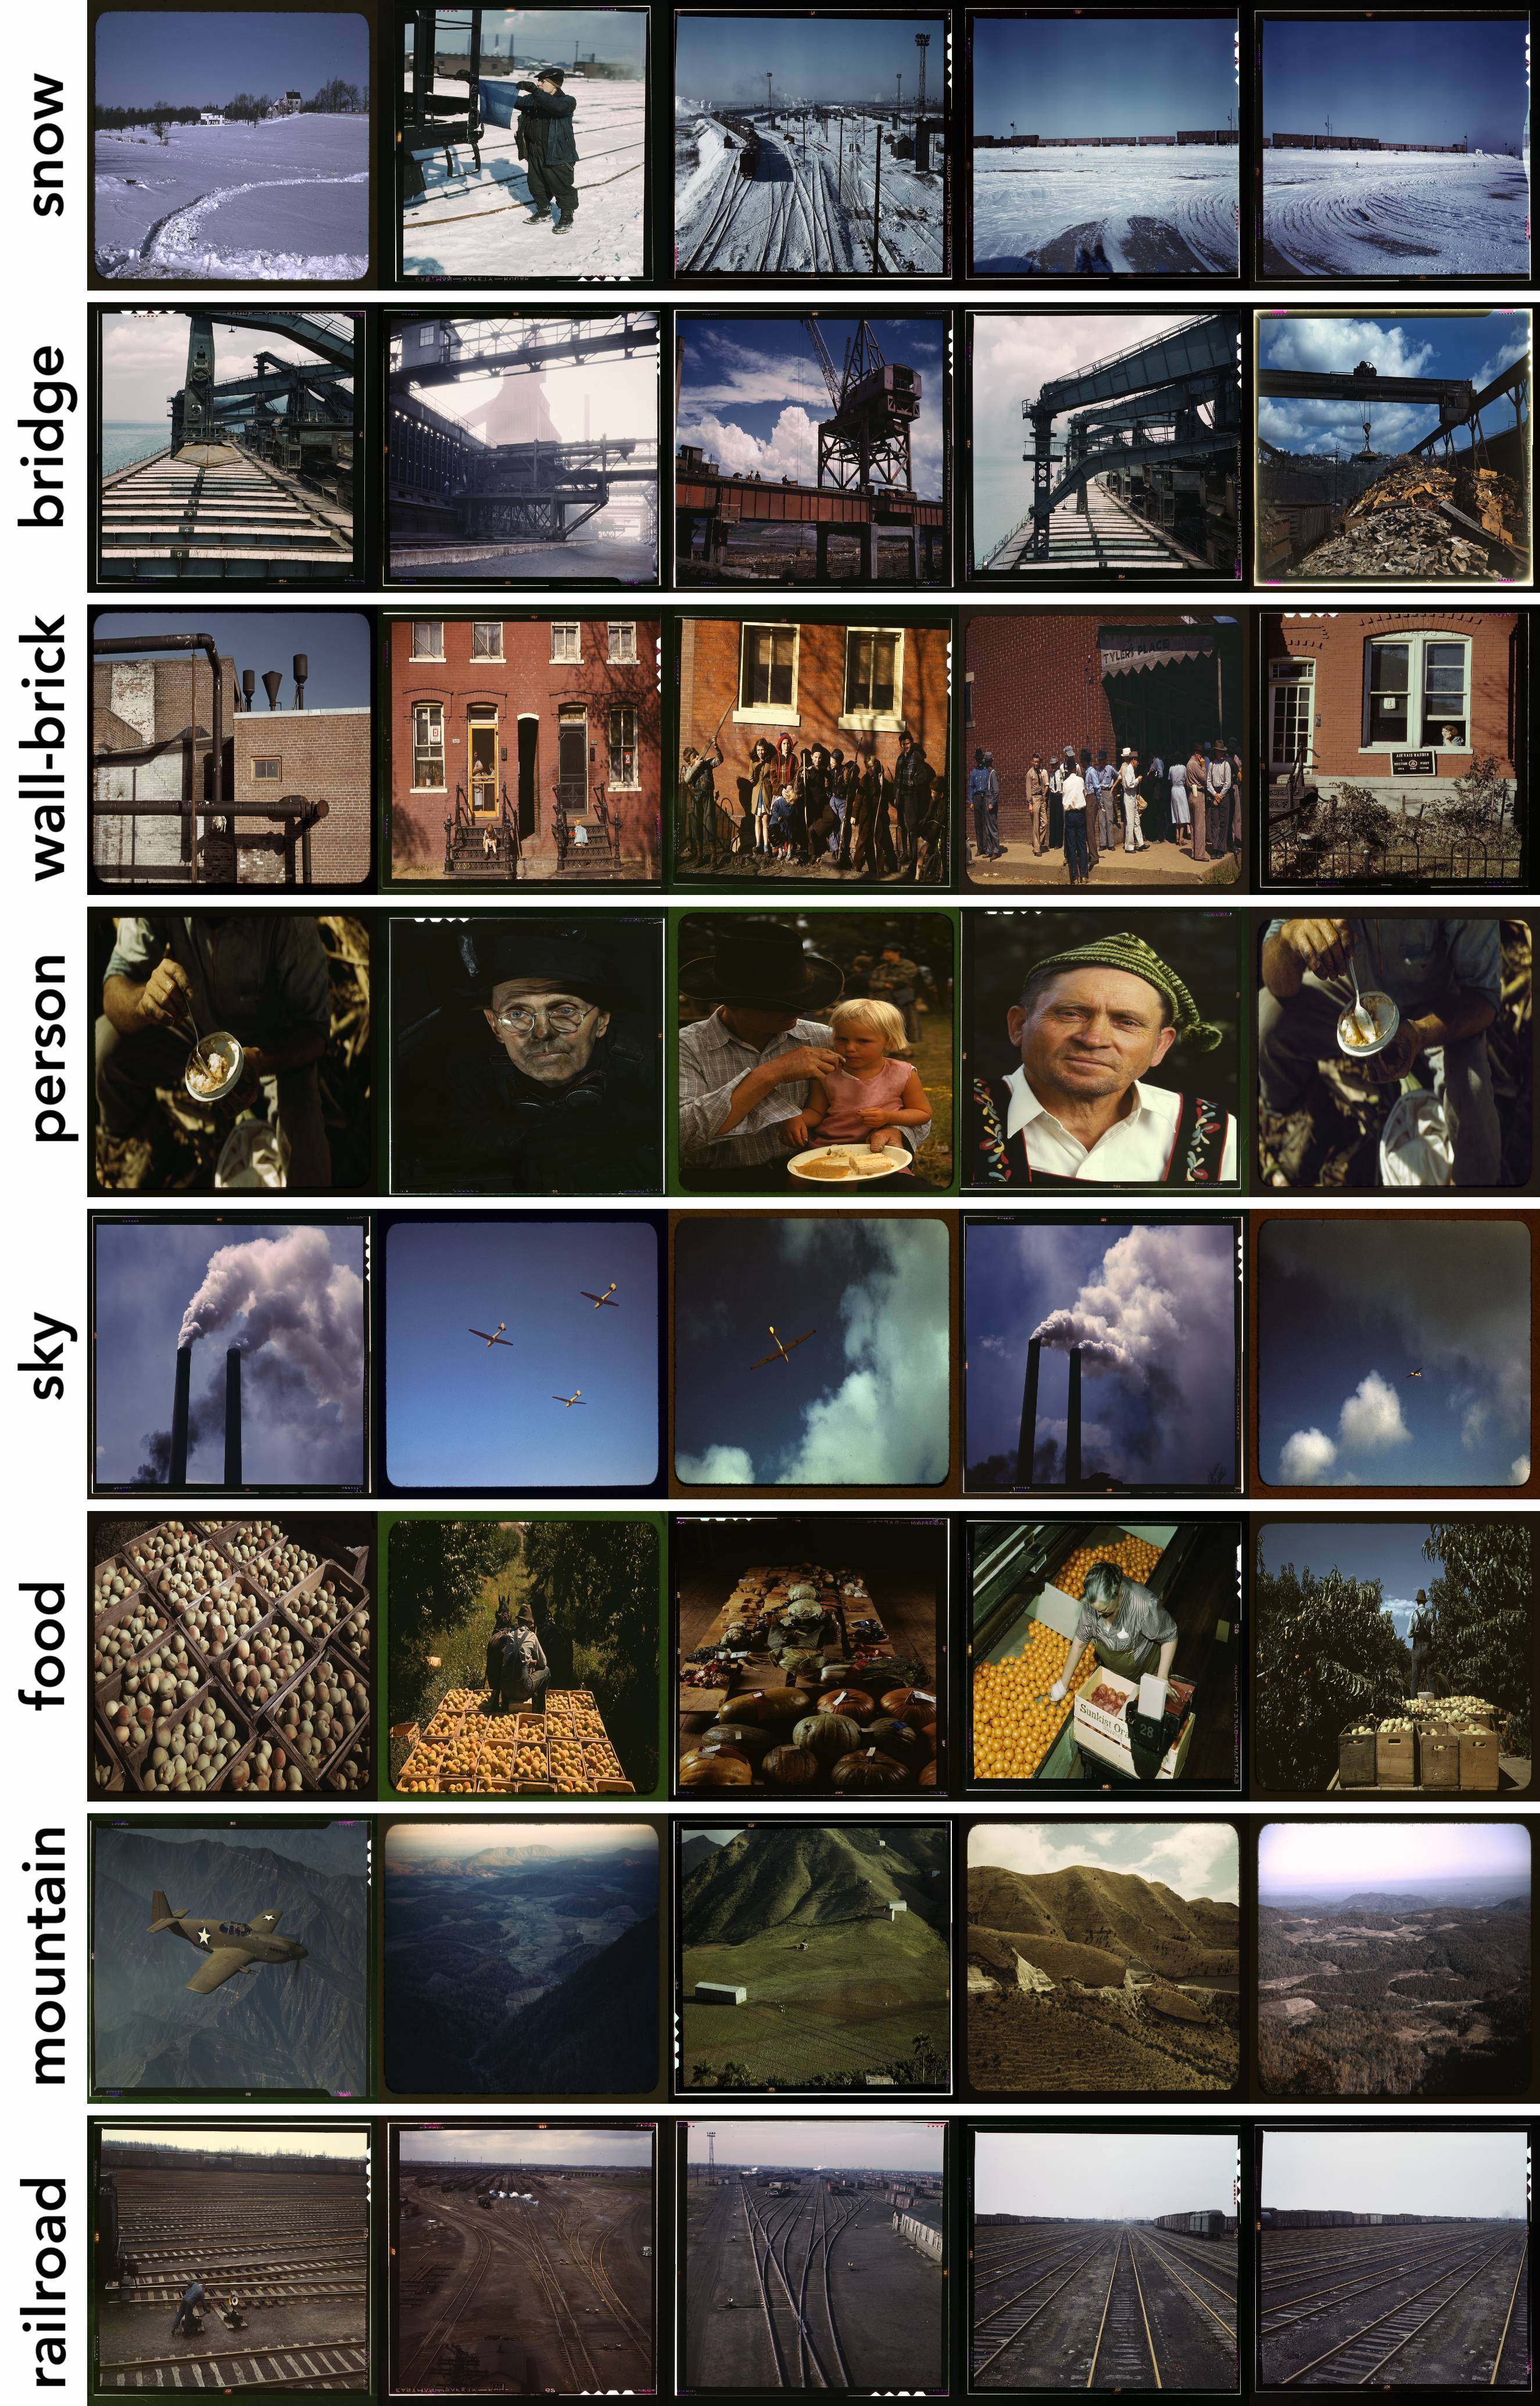
\includegraphics[height=0.9\textheight]{../figures/max_category_grid_labels.jpg}
\caption{Seven selected stuff types and the people category
shown with the five images from the FSA-OWI color photographs that are most
predicted to contain the given type. Uses the ResNet+FPN model provided by the
Detectron2 model zoo \protect\cite{wu2019detectron2}.
The only labels that appears the be falsely detected are in the third and
fifth bridge images, where construction equipment is falsely believed to be a
bridge.}
\label{fig:stuff}
\end{center}
\end{figure*}

\section{Evaluation} \label{sec:eval}

The annotation method described in Section~\secref{sec:method} was applied to the
entire corpus of 1610 color photographs from the FSA-OWI collection
\cite{trachtenberg1990reading}. An example of these are shown in
Figure~\ref{fig:stuff}. For the purpose of comparison,
two additional annotations were also computed.
Each photograph was tagged with detected objects and labelled with any object
that appeared with at least a probability of 85\% and for each photograph an
automatically detected caption was produced
(Figures~\ref{fig:things}-\ref{fig:captions} show examples of these
annotations).\footnote{Full replication code, data, and results are
available at: \url{https://github.com/statsmaths/fsa_color_analysis}.}
The annotations for each photograph were coded to indicate where the annotation
was accurately applied. A ``stuff'' region label was considered accurate if the
region was visible within the image and an object label was considered
accurate if the object existed somewhere in the image. A caption was considered
accurate if it could be considered true in a strictly literal sense. For
example, a caption saying that there are two people in an image that contains
three people was considered correct for our purpose. Because not all images
are guaranteed to include a region that falls above our threshold for inclusion,
we also recorded the percentage of images that had at least one
corresponding label (called recall in the results). The results are given in
Table~\ref{tab:results}.

\begin{table}[ht!]
\centering
\begin{tabular}{lccc}
 \hline
 & \textbf{Acc.} & \textbf{Recall} & \textbf{Unique Results} \\
 \hline
Stuff \& People & 97.5\% & 98.9\% & 1140 \\
Objects & 70.7\% & 37.3\% & 178 \\
Captions & 31.5\% & 100\% & 1040 \\
  \hline
\end{tabular}
\caption{Results of manually validated labels produced on the FSA-OWI color
photographs.}
\label{tab:results}
\end{table}

Both the close-analysis of the annotations in Figure~\ref{fig:stuff} illustrate
the efficacy of ``stuff'' region-based annotations for adding structured data to
historic image data. The object annotations do offer many useful features, but
have an error rate around 30\%, making them difficult to use without manual
validation. At the moment the captions are correct less than a third of the
time, and even the best captions fall far short of human-produced records. The
``stuff'' regions have an accuracy of 97.5\%; while public display of estimated
annotations should contain a note about their auto-generated nature, it is
possible to use these annotations without manual validation. The high accuracy
of the stuff-based annotation method does not come at the cost of producing only
uninteresting or unexpressive relations. In fact, the number of uniquely labelled
images is slightly higher than even the captions-based method, and labels were
found for nearly 99\% of all images. Looking manually at the results of the
most representative images, we see that the stuff-categories capture key
features of most of the image backgrounds and many of their foregrounds.

\section{Conclusions and Future Directions} \label{sec:conclude}

We have presented a method for the automated production of structured
data describing the content of photographic-corpora. The robustness and efficacy
of our method was shown through a case-study using 1610 documentary
photographs from the 1930s and 1940s. While other methods, such as
object-detection and automated caption generation, have the potential to provide
additional structured data, the generalizability of our approach offers a
strategy for algorithmically enriching large corpora of photographic materials
through structured data in order to facilitate access, discovery, and
exploration within and across collections.

The approach presented here offers several avenues for further extensions to
supply additional structured information to historic image corpora. First, there
are a number of ways that we could further encode information about the detected
regions. For example, recording the dominant colors of each region type or
indicating what part of an image a region is located. Secondly, it is possible
to develop a structured language for creating image captions from the structured
data. In connection with the first item, this would lead to captions such as a
``Photograph of two people, with a green mountain and blue sky in the
background''. This could produce image captions that, while more predictable
than techniques allowing for free-form language, are also significantly more
accurate. Finally, and most ambitiously, would be to construct a generic,
hierarchical version of a tagged object detection algorithm that simulates
the stuff-based regions. This would allow for a similar usage of
object-detection algorithms for the automated extraction of objects in the
foreground of an image without being constrained to narrowly defined categories
selected by current datasets.

\section{Acknowledgements}

Work supported by a National Endowment for the Humanities Digital Advancement
Grant (HAA-261239-18) and the Andrew W. Mellon Foundation's
\textit{Collections as Data: Part to Whole} initiative.

\nocite{*}
\section{Bibliographical References}\label{reference}
%\label{main:ref}

\bibliographystyle{lrec}
\bibliography{fsa-archive-cv}

% \section{Language Resource References}
% \label{lr:ref}
% \bibliographystylelanguageresource{lrec}
% \bibliographylanguageresource{languageresource}

\end{document}
